\documentclass[../main.tex]{subfiles}

\begin{document}

This project has been developed in the context of Xmipp and Scipion framework. The image processing algorithms have been implemented inside Xmipp, whilst the refinement logic has been implemented in the Xmipp's Scipion plugin.

The image processing part implemented in Xmipp has been named as \textit{swiftalign}, the union of the words \textit{swift} and \textit{align}. This name precisely describes the purpose of these programs: Fast image alignment. The \textit{swiftalign} framework implements two programs: \texttt{swiftalign\_train} and \texttt{swiftalign\_query}. 

These two programs, along other Xmipp programs, will be invoked from the Scipion protocol named as \textit{swiftres}. This protocol is used to implement the refinement logic. This means that it will be responsible of orchestrating calls to the image processing algorithms and provide an easy to use \gls{gui} for the end user.

\subsection{swiftalign}
Swiftalign is a framework of image processing programs that is part of the Xmipp image processing suite. These programs specialise in image alignment, this is, matching images considering all their in-plane transformations. Although several utility programs have been implemented during the development of this project, the most prominent ones are \texttt{swiftalign\_train} and \texttt{swiftalign\_query}. All the framework has been implemented in Python and it uses PyTorch library to accomplish computations such as common \gls{blas} routines and \glspl{fft}. This library is \gls{foss} and it is currently being developed by Facebook's AI Research lab. 

One of the key innovations of the project is the usage of state-of-the-art vector databases. These databases are implemented inside the FAISS library, which is also developed by Facebook. Therefore, a good integration between the former libraries is expected. 

Additionally, some file \gls{io} libraries are used to be able to read and write common file formats used in the context of \gls{cryoem}. This includes the \texttt{mrcfile} library used for reading images in \texttt{mrc} format and \texttt{starfile} library used for reading metadata files stored in \texttt{star} format. Both of these libraries are developed by the \gls{mrc}.

Many vector databases need to be trained before being populated. This training needs to be performed with data that resembles the actual data that is going to be used, so that the database can be structured optimally. This task is responsibility of \texttt{swiftalign\_train} which in rough terms performs a data augmentation of reference images to train a FAISS database.

Later this trained database is populated by \texttt{swiftalign\_query} using all possible in plane transformations of the reference gallery. Once populated, it is used to query experimental images and assign the estimated alignment parameters. Hence, the actual particle alignment will be carried out in this program.

\subsection{swiftres}
Both of the previous programs have been implemented as a \gls{cli} utility. This means that they can be invoked by the user from a command line prompt. However, the usage of parameters and invocation is not trivial. Therefore, a Scipion protocol was implemented that wraps these calls to perform a 3D refinement. This protocol, not only provides logic for determining invocation parameters but it also offers an easy to use \gls{gui}. This protocol is named as \textit{swiftres} and it will be introduced in this section.

The \gls{gui} of Scipion protocols is usually implemented as a form which lets the user choose the parameters for execution. These parameters may include the output of a previous step, a numeric value, toggle switch\dots When the appropriate parameters are selected, the protocol can be executed or saved for later use. In this case, the basic parameters to run \textit{swiftres} include the input particles, the initial volume(s), the resolution of the initial volume and the symmetry associated to the protein under study. A screenshot of this is displayed in Figure \ref{fig:4:form}.

\begin{figure}[hbpt]
    \centering
    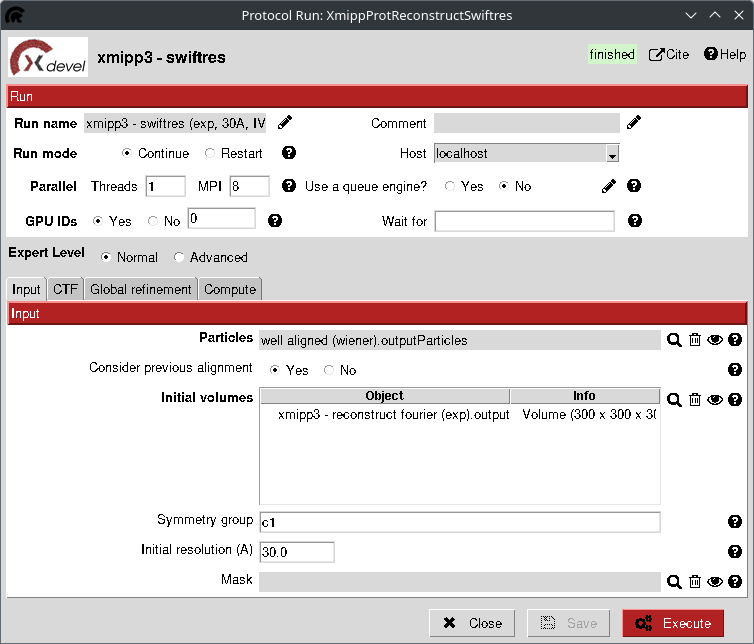
\includegraphics[width=.8\textwidth]{implementation/form}
    \caption{Screenshot of the user interface for running \textit{swiftres} protocol in Scipion}
    \label{fig:4:form}
\end{figure}

\end{document}
